\documentclass[text.tex]{subfiles}

\begin{document}
\section{Analysis of a quasicrystal with a circular window}
The methods for analysis of a general window from the previous section can be applied to the analysis of a circular window. First the hyper-window and the hypo-window need to be established. 

The quasicrystals based on the irrationality $\beta$ do intrinsically posses twelve-fold rotational symmetry. However this symmetry is only realized when the window posses twelve-fold rotational symmetry also. Which a circle naturally does. 

Formulas for inscribing and circumscribing a rhombus to a circle are rather simple, $\hat{\ell}$ and $\uhat{\ell}$ denote the sizes of the hyper-window and the hypo-window respectively, $R$ denotes the radius of the circle. 
$$\hat{\ell} = 4R \qquad \uhat{\ell} = \frac{15-3\beta}{4}R$$
The value for $\uhat{\ell}$ is actually an estimate. Precise formula contains $\sqrt{2}$ which is estimated by $6\beta - 21 \doteq 1.3923 < 1.4142 \doteq \sqrt{2}$ (unlike before this is a low estimate). The hypo-window is thus slightly smaller however unlike $\sqrt{2}$, $\uhat{\ell}\in M$.

With the hyper-window established, it is trivial to construct finite sections of a quasicrystal with a circular window. 

\begin{figure}[h!]
\centering
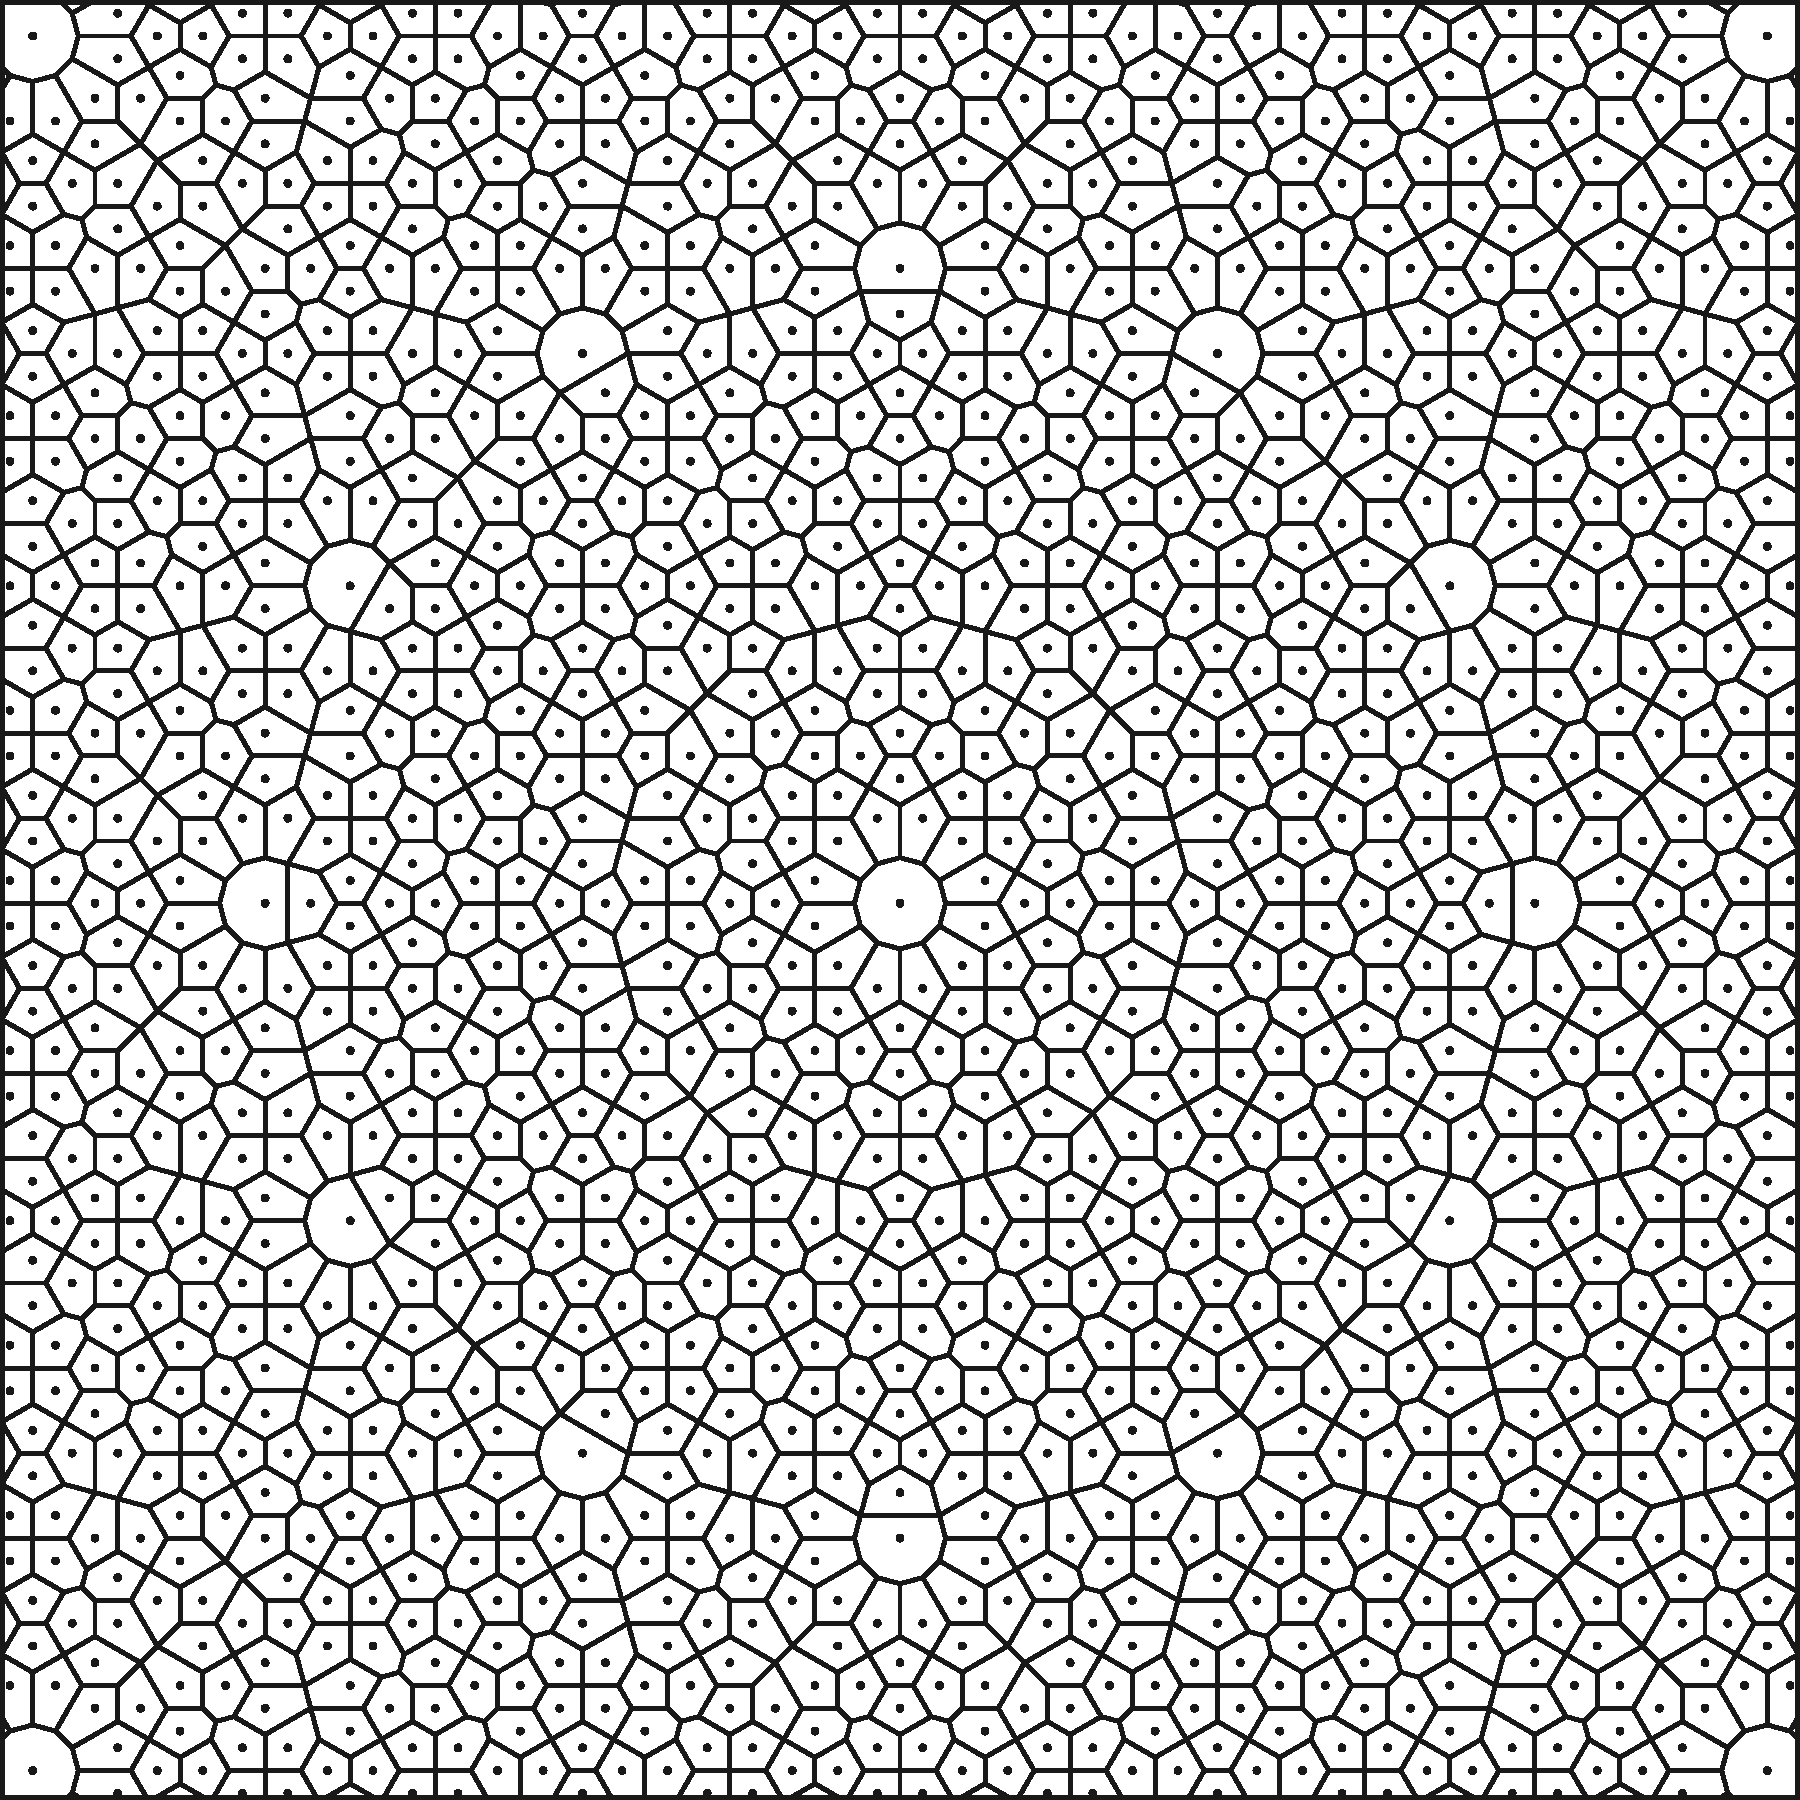
\includegraphics[width=0.88\textwidth]{circle/example}
\caption{Example of a finite section of a quasicrystal with a circular window (note the twelve-fold rotational symmetry).}
\end{figure}

However once attempting to catalog the voronoi polygons the computation was never able to finish neither memory-wise nor time-wise. Therefore the aim of further work is to parallelize the program and properly finish the analysis of quasicrystals with circular windows. 
\end{document}
